\section*{vw4tools }

Tools and utilities for Virtual\+Wisdom4

At current, V\+W4\+Tools is a script or two, plus one big jar file. vw4tool.\+jar allows a user to import a text file in one of several formats and output an Entity import J\+S\+O\+N for Virtual\+Wisdom4.

\section*{Running Java }

In this document, it is assumed \char`\"{}java\char`\"{} runs from the command prompt. In some cases, this isn't true. Windows users, for example, may need to change their usage, from\+: \begin{DoxyVerb}java -jar vw4tool.jar ...
\end{DoxyVerb}


to\+: \begin{DoxyVerb}java.exe -jar vw4tool.jar ...
\end{DoxyVerb}


In both cases, if the \char`\"{}java\char`\"{} (or java.\+exe) executable is not available on the user's \char`\"{}path\char`\"{} or list of locations wherein to find a binary/executable, the user will need to type the full pathname to the java executable.

Macintosh O\+S\+X users can simply type \char`\"{}java\char`\"{}\+: \begin{DoxyVerb}java -jar vw4tool.jar ...
\end{DoxyVerb}


A U\+N\+I\+X (or unix-\/like) user may need to type /opt/local/bin/java or similar\+: \begin{DoxyVerb}/opt/local/bin/java -jar vw4tool.jar ...
\end{DoxyVerb}


A Windows user may need to type a full pathname such as\+: \begin{DoxyVerb}"C:\Program Files (x86)\Java\jre7\bin\java.exe" -jar vw4tool.jar ...
\end{DoxyVerb}


In all cases, where I type merely \char`\"{}java\char`\"{}, make sure you replace that with however the invocation details are for your platform.

To confirm you've found a working Java Runtime Environment, use the \char`\"{}help\char`\"{} command to as vw4tool.\+jar what version it is\+: \begin{DoxyVerb}java -jar vw4tool.jar --help
Usage: vw4tool -V|--version|-H|--help
     : vw4tool --read <filename>|--input <filename> | -r <filename> | -i <filename>
   ie: vw4tool --read import.json
   ie: vw4tool -r import.json
\end{DoxyVerb}


note\+: many commands have shorter versions. \char`\"{}-\/-\/version\char`\"{} (with two \char`\"{}-\/\char`\"{}) is the same as \char`\"{}-\/\+V\char`\"{} (with one dash). Pay special attention to case. Uppercase \char`\"{}\+N\char`\"{} is different from lowercase \char`\"{}n\char`\"{}.

\section*{Common Usage }

\begin{DoxyVerb}java -jar vw4tool.jar  -N localfile1.txt -N localfile2.txt -N localfile3.txt -oexample.json
\end{DoxyVerb}


or \begin{DoxyVerb}java -jar vw4tool.jar  -N localfile1.txt -N localfile2.txt -N localfile3.txt -oOrderedTuples.csv
awk -f csv-to-json.awk OrderedTuples.csv > example.json
\end{DoxyVerb}


This is the most common usage, here as a reference. Notice that although this shows E\+I\+T\+H\+E\+R Ordered\+Tuples.\+csv or a J\+S\+O\+N file being created, both could be created by multiple \char`\"{}-\/o\char`\"{} options. Notice also that \char`\"{}-\/o\char`\"{} is \char`\"{}cuddled\char`\"{} to the filename after it. No spaces, but this should change in the future to avoid ambiguity.

\section*{Overview }

In general, collection and conversion looks like the following diagram\+:

\begin{center}

\begin{DoxyImageNoCaption}
  \mbox{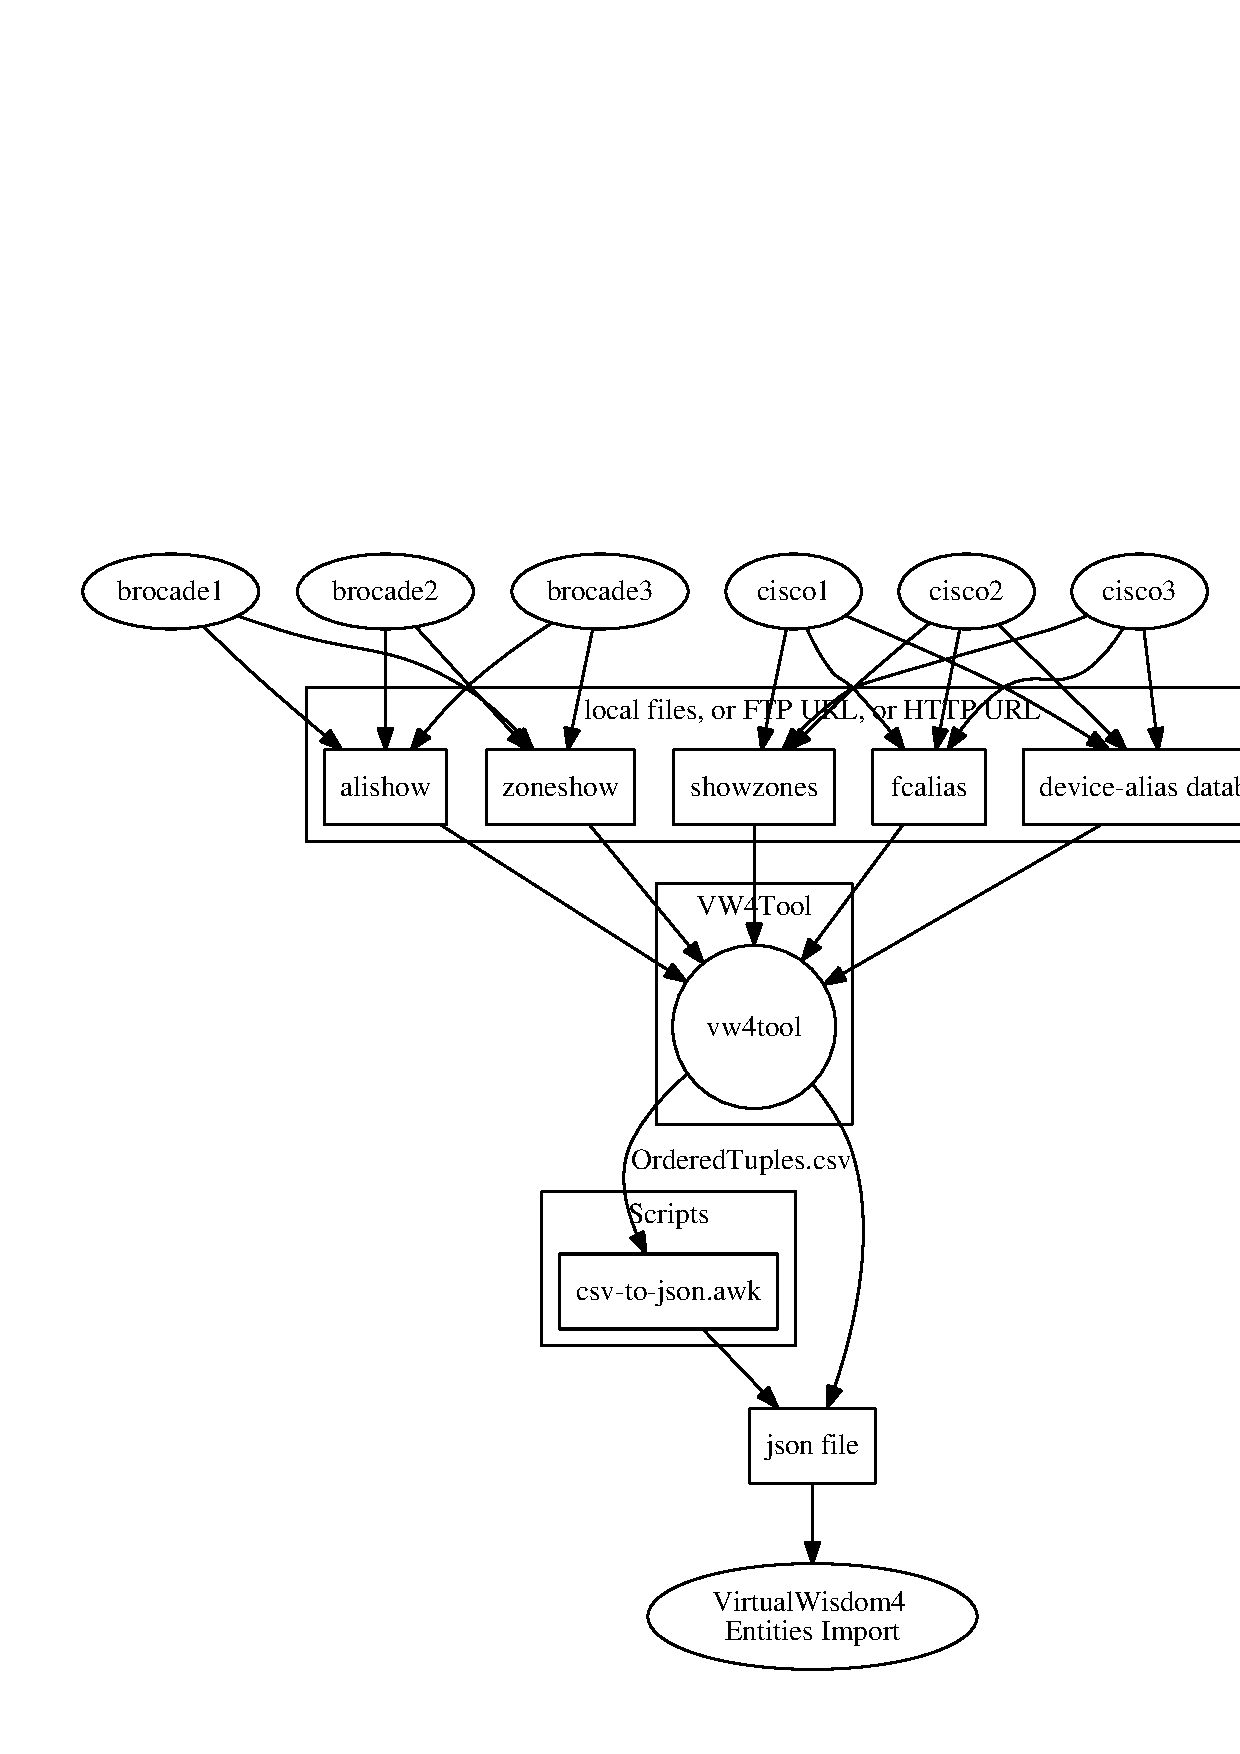
\includegraphics[width=\textwidth,height=\textheight/2,keepaspectratio=true]{dot_inline_dotgraph_1}}
\end{DoxyImageNoCaption}
\end{center}


\section*{Import of F\+T\+P or H\+T\+T\+P Data }

V\+W4\+Tools uses the U\+R\+L\+Data\+Source functionality to open a stream from a H\+T\+T\+P or F\+T\+P server; this means that the files it parses can be stored on a local filesystem, a F\+T\+P server, and an H\+T\+T\+P server as constant data, or can be the result of a C\+G\+I program on an H\+T\+T\+P server. Less common, a local fil emay also be mounted as a F\+U\+S\+E filesystem, allowing even \char`\"{}local\char`\"{} data to be generated like a C\+G\+I program.

In order to draw a text stream from a F\+T\+P server or H\+T\+T\+P server, merely use a R\+F\+C-\/1738-\/compliant U\+R\+L to indicate these two sources\+: \begin{DoxyVerb}(ftp|http)://{user{:password@@}server{:port}/pathname/to/resource
\end{DoxyVerb}


for example\+:

(basic user/pass\+: user = scott, pass = T1ger, host = ftp.\+example.\+com, subdir = . , file = nicknames.\+txt \begin{DoxyVerb}java -jar vw4tool.jar --nickname=ftp://scott:T1ger@@ftp.example.com/nicknames.txt
\end{DoxyVerb}


(basic user/pass\+: user = scott, pass = T1ger, host = ftp.\+example.\+com, subdir = /users/local/\+Scott\+Adams/ , file = aliases.\+text \begin{DoxyVerb}java -jar vw4tool.jar --nickname=ftp://scott:T1ger@@ftp.example.com/%2fusers/local/ScottAdams/aliases.text
\end{DoxyVerb}


(basic user/pass\+: user = anonymous, pass = scott@uberserver.\+net, host = ftp.\+example.\+com, subdir = examples , file = aliases \begin{DoxyVerb}java -jar vw4tool.jar -N ftp://anonymous:scott%2Fuberserver.net@@ftp.example.com/examples/aliases
\end{DoxyVerb}


(basic http\+: host = www.\+example.\+com, subdir = . , file = aliases \begin{DoxyVerb}java -jar vw4tool.jar --nickname=http://www.example.com/aliases
\end{DoxyVerb}


(basic H\+T\+T\+P G\+E\+T\+: host = www.\+example.\+com, subdir = . , path=/cgi-\/bin/fetch.cgi, some parameters \begin{DoxyVerb}java -jar vw4tool.jar --nickname=http://www.example.com/cgi-bin/fetch.cgi?now=20140901&realm=WEST&group=production
\end{DoxyVerb}


N\+O\+T\+E\+: \char`\"{}-\/-\/nickname=\char`\"{} and \char`\"{}-\/\+N\char`\"{} are functionally identical; \char`\"{}-\/-\/nickname=\char`\"{} may offer a slight beefit in more clearly self-\/documenting the behavior of the commandline option.

\section*{Import of Local Text File }

The most common usage is local text files representing the metadata of the local environment. This is done by offering a R\+F\+C-\/1738-\/compliant local file U\+R\+L\+: \begin{DoxyVerb}file://pathname/to/resource
\end{DoxyVerb}


Note that if the \char`\"{}file\+://\char`\"{} is not given, and no \char`\"{}protocol\char`\"{} (ie \char`\"{}file\+://\char`\"{}) is given, vw4tool will warn you about this but try the local {\tt file\+://} protocol prefix for you

for example\+:

(local file in subdir ./files/aliases) \begin{DoxyVerb}java -jar vw4tool.jar --nickname=file://files/aliases
java -jar vw4tool.jar --nickname=files/aliases
\end{DoxyVerb}


(local file in subdir /\+Full/\+Path/files/aliases) \begin{DoxyVerb}java -jar vw4tool.jar --nickname=file:///Full/Path/files/aliases
java -jar vw4tool.jar --nickname=/Full/Path/files/aliases
\end{DoxyVerb}


\section*{Specifying Formats }

The user doesn't need to speficy the format of a file; vw4tool will try the file at the same time across many different parsers and see which one can make sense of it. Unfortunately, the parsers cannot always chew through any user-\/interface codes (such as \char`\"{}press any key to continue\char`\"{}) and preamble (the verbose text trash before the actual zone or aliases or such). Trimming that to a minimum offers a better chance of parsing the file.

The corollary to this is that if a file doesn't seem to parse, yet it seems like it should, remove anything before or after the actual content, and confirm that it was collected in a non-\/interactive method. If the user ever needs to \char`\"{}press any key for more\char`\"{}, chances are, the parsed result will be either partial, or none at all.

\section*{Multiple Inputs }

These input formats can be mixed. For example \begin{DoxyVerb}java -jar vw4tool.jar --nickname=http://www.example.com/cgi-bin/fetch.cgi?now=20140901&realm=WEST&group=production -N local.txt -N file:///Users/allanc/aliases.dad -N morefiles.txt
\end{DoxyVerb}


\section*{Outputs }

vw4tool will either generate an Ordered\+Tuples.\+csv file (if that specific filename is given on the \char`\"{}-\/o\char`\"{} option) or a json file (any other putput filename). Or both\+: \begin{DoxyVerb}java -jar vw4tool.jar  -N local.txt -oOrderedTuples.csv -oexample.json
\end{DoxyVerb}


N\+O\+T\+E\+: giving no filename sends the output to stdout\+: \begin{DoxyVerb}java -jar vw4tool.jar  -N local.txt -o
\end{DoxyVerb}


For this reason, the following two commands do different things\+: \begin{DoxyVerb}java -jar vw4tool.jar  -N local.txt -oexample.json
java -jar vw4tool.jar  -N local.txt -o example.json
\end{DoxyVerb}


Stdout can be represented as \char`\"{}-\/\char`\"{}; the following two commands do the same thing\+: \begin{DoxyVerb}java -jar vw4tool.jar  -N local.txt -o
java -jar vw4tool.jar  -N local.txt -o-
\end{DoxyVerb}


This behavior may disappear in future. Please try to use \char`\"{}-\/\char`\"{} to print the result to stdout\+: \begin{DoxyVerb}java -jar vw4tool.jar  -N local.txt -N (another) --nickname=(another) -o-
\end{DoxyVerb}


\section*{Proprietary Intellectual Property }

With the exception of samples/import01.\+json, all files and content are based on the same level of access to the product enjoyed by a customer. Implicitly, no private information is shared, all of this content (save the one file) is based on empirical discovery, and could change overnight. 